\section{Contexte}

\subsubsection{Un peu d’histoire}

Tout commence en 1736, avec Léonhard Euler, lorsqu’il s’intéressa au célèbre problème des sept ponts de Königsberg : existe-t-il un moyen de traverser tous les ponts de la figure une seule et unique fois ? Pour répondre à cette question qui semble à première vue anodine, Euler a initié la théorie de ce que l’on appellera par la suite la topologie algébrique : un pan des mathématiques qui met de côté les longueurs, les droites et tout ce qui s’ensuit. Nous devons notamment à celui-ci la formule servant aujourd’hui d’invariant topologique sur un cube : $S - C + F = 2$, avec respectivement $S$ le nombre de sommets, $C$ de côtés et $F$ de faces.

\begin{figure}[H]
\centering
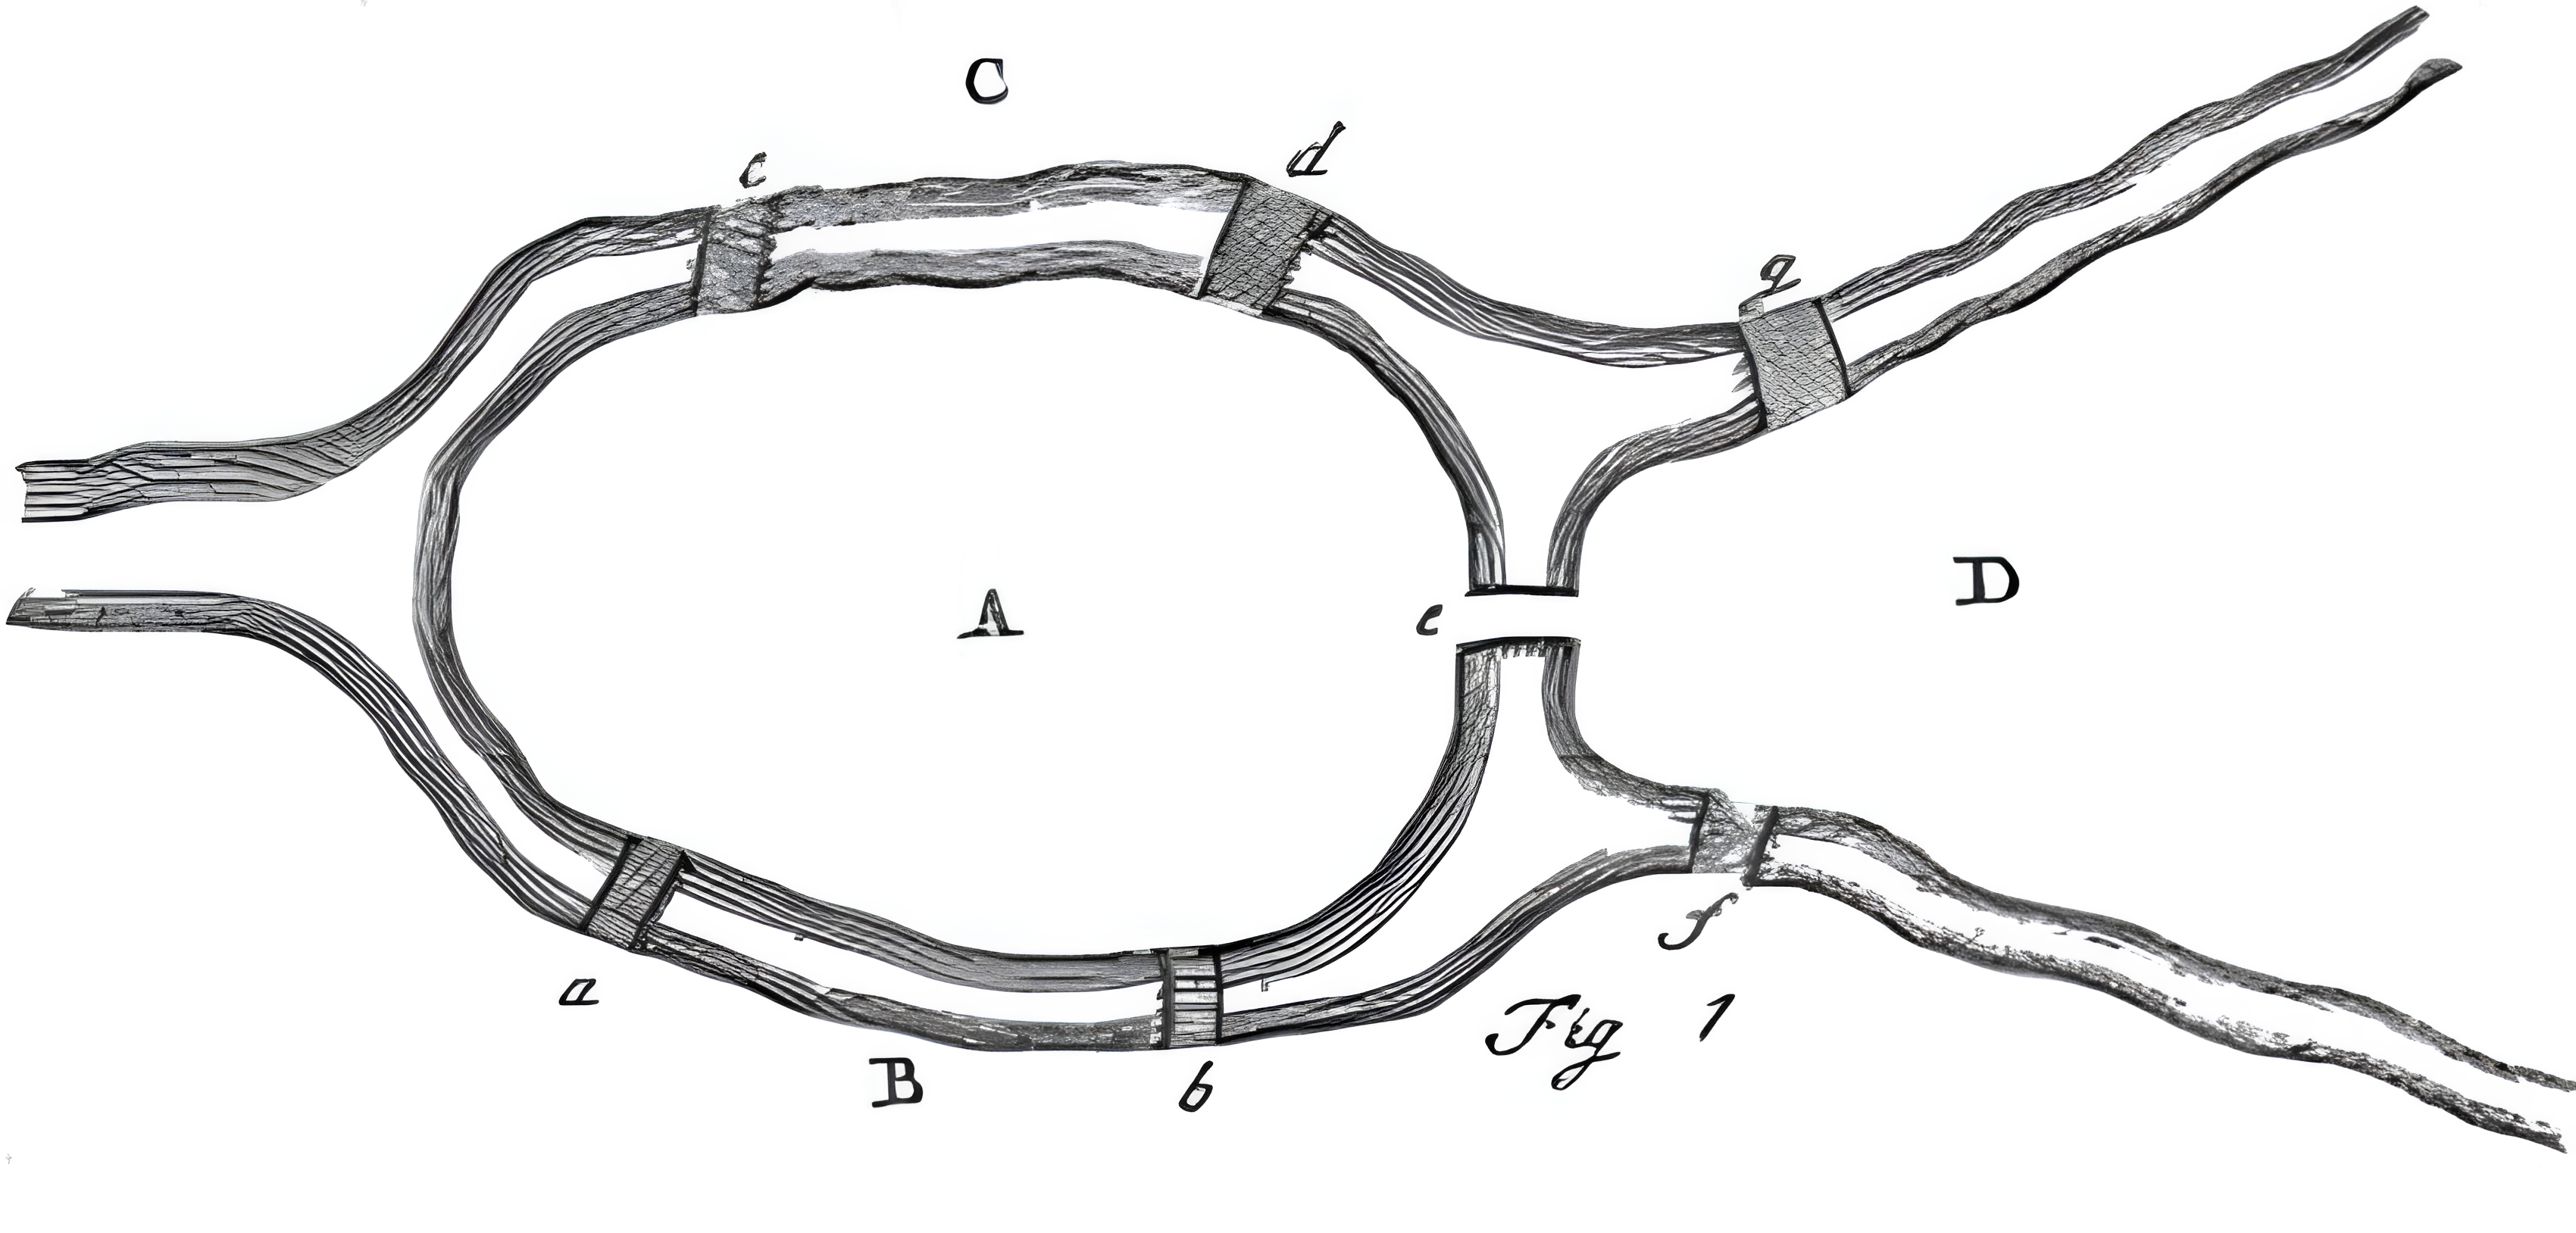
\includegraphics[width=0.4\textwidth]{pictures/SevenBridges.png}
\caption{Illustration du problème des sept ponts de Königsberg}
\label{img:seven-bridges}
\end{figure}

Au cours du XIX\textsuperscript{e} siècle, certains grands mathématiciens ont eu l’occasion de poser une pierre à l’édifice de ce qu’est l’actuelle topologie. Bernhard Riemann a travaillé sur la géométrie complexe, dont certains résultats sont très liés à notre domaine. Enrico Betti a, quant à lui, étudié la notion de connexité. Cela lui a permis de donner son nom à un invariant topologique : les nombres de Betti. Felix Klein a été à l’initiative du programme d’Erlangen. Ce dernier a pour but d’étudier la géométrie, et en particulier les différentes géométries, d’un point de vue global. C’est ainsi qu’ont été introduites les notions d’actions de groupe et d’invariants topologiques.

C’est en 1895 que la topologie algébrique commence à ressembler à ce que nous connaissons, notamment avec les travaux d’Henri Poincaré et son livre \textit{Analysis Situs}. C’est en grande partie à lui que l’on doit les résultats sur lesquels nous allons nous intéresser dans ce rapport, tels que le groupe fondamental. Par exemple, il s’est posé la question suivante : les nombres de Betti peuvent-ils représenter une surface, topologiquement parlant ? Nous reconnaissons ici les premiers questionnements sur les invariants topologiques.

Ce dernier mathématicien n’a malheureusement pas découvert tout le potentiel algébrique existant derrière les invariants topologiques qu’il a étudiés, et notamment les nombres de Betti. Cette découverte, de laquelle découleront les groupes d’homologie, a été initiée par Emmy Noether en 1926. C’est également à elle que nous devons le formalisme actuel de l’algèbre, de la topologie ainsi que de la topologie algébrique.

\subsubsection{Contexte et objectifs}

Dans la branche des mathématiques fondamentales, nous cherchons à établir des théorèmes de classification, ou autrement dit des relations d’équivalence sur un ensemble d’objets. Nous pouvons prendre l’exemple des espaces vectoriels finis, qui sont classifiés à isomorphisme près par leur dimension.

C’est dans le même espoir que la topologie algébrique se caractérise : l’objectif est de classifier les espaces topologiques homéomorphes les uns aux autres. Il a cependant été démontré \cite{homeoImpossible} qu’il est impossible d’effectuer un tel résultat. Alors, la topologie algébrique se retrouve en quête d’outils permettant une classification de ces espaces, prenant en compte les invariants topologiques.

\bigskip Ce mémoire, issu de trois mois de recherche et de lecture, est décomposé en deux grands chapitres, chacun centré sur un invariant topologique. Historiquement, ils ont été introduits comme étant une potentielle solution à notre problème de classification, mais nous savons de nos jours qu'ils ne suffisent pas.

Plus précisément, le premier chapitre sert d'introduction, où l'on expose le contexte et les notions préliminaires nécessaires pour la compréhension de la suite. Le second chapitre se concentre sur le \emph{groupe fondamental}, un outil puissant mais dont l'utilisation reste complexe. Bien que celui-ci offre une visualisation assez évidente, la théorie est tout autre, notamment à cause des notions complexes nécessaires à y introduire. Le groupe fondamental du cercle, dont l'étude recouvre plusieurs pages de résultats et de preuves, en est un parfait exemple. Le troisième chapitre se focalise sur les \emph{groupes d'homologies}, un outil qui vient aux antipodes du groupe fondamental. Leur usage sont bien plus efficaces, preuves à l'appui, et permettent d'étudier des espaces plus complexes. Néanmoins, l'intuition est ici limitée, notamment car la représentation visuelle de l'outil ne se fait que peu (voire pas). Ce chapitre est découpé en trois sections, chacune étant centrée sur une homologie en particulier. Ceci permettra de mettre en lumière leurs différences ainsi que leurs points communs : nous verrons en particulier qu'elles sont toutes identiques à isomorphisme près.

Nous retrouverons en annexe deux petits chapitres supplémentaires. Le premier donne des exemples de calculs que nous pouvons effectuer avec l'homologie simpliciale (voir chapitre \ref{chp:homology}). Le second est une brève introduction à la théorie des catégories, une branche des mathématiques sur laquelle se fonde la topologie algébrique (d'où l'utilisation des flèches).